\documentclass[12pt]{article}

% Load packages
\usepackage{url}  % Formatting web addresses
\usepackage{ifthen}  % Conditional
\usepackage{multicol}   %Columns
\usepackage[utf8]{inputenc} %unicode support
\usepackage{amsmath}
\usepackage{amssymb}
\usepackage{epsfig}
\usepackage{epstopdf}
\usepackage{graphicx}
\usepackage[margin=0.1pt,font=footnotesize,labelfont=bf]{caption}
\usepackage{setspace}
%\usepackage{longtable}
\usepackage{colortbl}
%\usepackage{palatino,lettrine}
%\usepackage{times}
%\usepackage[applemac]{inputenc} %applemac support if unicode package fails
%\usepackage[latin1]{inputenc} %UNIX support if unicode package fails
\usepackage[wide]{sidecap}
%\usepackage[authoryear,round,comma,sort&compress]{natbib}
\usepackage[square,sort,comma,numbers,sort&compress]{natbib}
%\usepackage[authoryear,round]{natbib}
\usepackage{supertabular}
\usepackage{simplemargins}
\usepackage{fullpage}
\usepackage{comment}
\usepackage{lineno}
%\usepackage{chicago}
\usepackage{textcomp}
\usepackage{multirow}
\usepackage{amsmath}
%\usepackage[linesnumbered,lined,boxed,commentsnumbered]{algorithm2e}
\DeclareMathOperator*{\argmin}{\arg\!\min}

%\usepackage{algorithm2e}
%\usepackage{algpseudocode}
%\usepackage[space]{cite}
\urlstyle{rm}

%\textwidth = 6.50 in
%\textheight = 9.5 in
%\oddsidemargin =  0.0 in
%\evensidemargin = 0.0 in
%\topmargin = -0.50 in
%\headheight = 0.0 in
%\headsep = 0.25 in
%\parskip = 0.15in
%\linespread{1.75}
\doublespace

%\bibliographystyle{chicago}
\bibliographystyle{plos2009}

\makeatletter
\renewcommand\subsection{\@startsection
	{subsection}{2}{0mm}
	{-0.05in}
	{-0.5\baselineskip}
	{\normalfont\normalsize\bfseries}}
\renewcommand\subsubsection{\@startsection
	{subsubsection}{2}{0mm}
	{-0.05in}
	{-0.5\baselineskip}
	{\normalfont\normalsize\itshape}}
\renewcommand\section{\@startsection
	{subsection}{2}{0mm}
	{-0.2in}
	{0.05\baselineskip}
	{\normalfont\large\bfseries}}
\renewcommand\paragraph{\@startsection
	{paragraph}{2}{0mm}
	{-0.05in}
	{-0.5\baselineskip}
	{\normalfont\normalsize\itshape}}
\makeatother

%Review style settings
%\newenvironment{bmcformat}{\begin{raggedright}\baselineskip20pt\sloppy\setboolean{publ}{false}}{\end{raggedright}\baselineskip20pt\sloppy}

%Publication style settings

% Single space'd bib -
\setlength\bibsep{0pt}

\renewcommand{\rmdefault}{phv}\renewcommand{\sfdefault}{phv}
\newcommand{\norm}[1]{\left\lVert#1\right\rVert}

% Change the number format in the ref list -
\renewcommand{\bibnumfmt}[1]{#1.}

% Change Figure to Fig.
\renewcommand{\figurename}{Fig.}

% Begin ...
\begin{document}
\begin{titlepage}
{\par\centering\textbf{\Large {Toward a Genome Scale Dynamic Model of Cell Free Protein Synthesis in \emph{Escherichia~coli}}}}
\vspace{0.05in}
{\par \centering \large{Nicholas Horvath, Michael Vilkhovoy, James Swartz$^{1}$ and Jeffrey D. Varner$^{*}$}}
\vspace{0.10in}
{\par \centering {School of Chemical and Biomolecular Engineering}}
{\par \centering {Cornell University, Ithaca NY 14853}}
\vspace{0.1in}
{\par \centering {$^{1}$School of Chemical Engineering}}
{\par \centering {Stanford University, Stanford, California 94305}}
{\par \centering \textbf{Running Title:}~Dynamic model of cell free protein synthesis}
\vspace{0.1in}
{\par \centering \textbf{To be submitted:}~\emph{Scientific~Reports}}
\vspace{0.5in}
{\par \centering $^{*}$Corresponding author:}
{\par \centering Jeffrey D. Varner,}
{\par \centering Professor, School of Chemical and Biomolecular Engineering,}
{\par \centering 244 Olin Hall, Cornell University, Ithaca NY, 14853}
{\par \centering Email: jdv27@cornell.edu}
{\par \centering Phone: (607) 255 - 4258}
{\par \centering Fax: (607) 255 - 9166}
\end{titlepage}
\date{}
\thispagestyle{empty}
\pagebreak
%%%%%%%%%%%%%%%%%%%%%%%%%%%%%%%%%%%%%%%%%%%%%%%%%%%%%%%%%%%%%%%%%%%%%%%%%%%%%%%%%%%%%%%%%%%%%%%%%%%%%%%%%%%
%%%%%%%%%%%%%%%%%%%%%%%%%%%%%%%%%%%%%%%%%%%%%%%%%%%%%%%%%%%%%%%%%%%%%%%%%%%%%%%%%%%%%%%%%%%%%%%%%%%%%%%%%%%
\section*{Abstract}
Fill me in.


%We further tested the predictive power of the coagulation model parameters against data not used in training, and found good agreement between simulations and experimental measurements. Lastly, we tested the performance of DOPS on commonly used test functions for global optimization and on published biochemical parameter estimation benchmark problems. For the wide range of problems that we considered, DOPS outperformed other meta-heuristic approaches despite a limited number of function evaluations.

\vspace{0.1in}
{\noindent \textbf{Keywords:}~Biochemical engineering, systems biology, cell free protein synthesis}

% Extra abstract
% Mathematical modeling of biological systems with multiple feed back loops is one such area where parameter estimation is a difficult non-linear optimization problem. This difficulty is further compounded when dealing with parameter vectors of high dimensions.

%In this study, we present the dynamically dimensioned particle
%a novel meta-heuristic approach that combines a variant of particle swarm optimization (PSO) along with dynamically dimensioned search (DDS) to obtain near optimal solutions of high dimensional biochemical networks within a relatively few function evaluations.
%We use a particle swarm optimization technique that uses multi-swarms to generate candidate vectors which are then greedily updated using DDS by dynamically varying the perturbed parameter dimensions. We tested this algorithm (25 trials with 4000 function evaluations in each trial) on a biochemical network of coagulation (148 parameters and 92 species) and compared it's performance against other meta-heuristics like Differential Evolution (DE), Particle Swarm Optimization (PSO), Simulated Annealing (SA) and also against DDS alone. The new algorithm outperforms all the other meta-heuristics on the coagulation model. The parameter vectors obtained using this approach fit the experimental data well and also make accurate enough predictions on unseen experimental data. We also performed this comparison on commonly used test functions (Ackley and Rosenbrock) for global optimization and found the same behavior. Further we used two recently published benchmark problems, a genome wide kinetic model with 1759 parameters and a metabolic model of Chinese Hamster Ovary cells with 117 parameters to evaluate the performance of our approach. We  surprisingly performed well on these benchmarks and obtained the nominal parameter vector with just 4000 function evaluations in both cases.

\pagebreak

\setcounter{page}{1}

% Uncomment in production -
%\linenumbers


\section*{Introduction}

Mathematical modeling has long contributed to our understanding of metabolism. Decades before the genomics revolution, mechanistically, structured metabolic models arose from the desire to predict microbial phenotypes resulting from changes in intracellular or extracellular states \citep{1976_fredrickson_BiotechBioeng}.
The single cell \textit{E. coli} models of Shuler and coworkers pioneered the construction of large-scale, dynamic metabolic models that incorporated multiple, regulated catabolic and anabolic pathways constrained by experimentally determined kinetic parameters \citep{1984_domach_shuler_BiotechBioeng_01}.
Shuler and coworkers generated many single cell kinetic models, including single cell models of eukaryotes \citep{1989_steinmeyer_shuler_ChemEngSci,1992_wu_shuler_AnnNYAcadSci}, minimal cell architectures \citep{2004_castellanos_shuler_PNAS}, as well as DNA sequence based whole-cell models of \textit{E. coli} \citep{2008_atlas_shuler_IETSysBio}.
Conversely, highly abstracted kinetic frameworks, such as the cybernetic framework, represented a paradigm shift, viewing cells as growth-optimizing strategists \citep{1985_dhurjati_ramkrishna_tsao_BiotechBioeng}.
Cybernetic models have been highly successful at predicting metabolic choice behavior, e.g., diauxie behavior \citep{1986_kompala_ramkrishna_tsao_BiotechBioeng}, steady-state multiplicity \citep{2012_kim_ramkrishna_BiotechProg}, as well as the cellular response to metabolic engineering modifications \citep{1999_varner_ramkrishna_MetaEng}.
Unfortunately, traditional, fully structured cybernetic models also suffer from an identifiability challenge, as both the kinetic parameters and an abstracted model of cellular objectives must be estimated simultaneously.
However, recent cybernetic formulations from Ramkrishna and colleagues have successfully treated this identifiability challenge through elementary mode reduction~\cite{2009_song_ramkrishna_BiotechBioeng,Song:2011aa}.

In the post genomics world, large-scale stoichiometric reconstructions of microbial metabolism popularized by static, constraint-based modeling techniques such as flux balance analysis (FBA) have become standard tools \citep{2012_lewis_palsson_NatRevMicrobio}.
Since the first genome-scale stoichiometric model of \textit{E. coli}, developed by Edwards and Palsson \citep{2000_edwards_palsson_PNAS}, well over 100 organisms, including industrially important prokaryotes such as \textit{E. coli} \citep{Feist:2007aa} or \textit{B. subtilis} \citep{Oh:2007aa}, are now available \citep{2009_feist_palsson_NatRevMicrobio}.
Stoichiometric models rely on a pseudo-steady-state assumption to reduce unidentifiable genome-scale kinetic models to an underdetermined linear algebraic system, which can be solved efficiently even for large systems.
Traditionally, stoichiometric models have also neglected explicit descriptions of metabolic regulation and control mechanisms, instead opting to describe the choice of pathways by prescribing an objective function on metabolism.
Interestingly, similar to early cybernetic models, the most common metabolic objective function has been the optimization of biomass formation \citep{2002_ibarra_edwards_palsson_Nat}, although other metabolic objectives have also been estimated \citep{2007_schuetz_sauer_MolSysBio}.
Recent advances in constraint-based modeling have overcome the early shortcomings of the platform, including capturing metabolic regulation and control \citep{2013_hyduke_lewis_palsson_MolBioSys}.
Thus, modern constraint-based approaches have proven extremely useful in the discovery of metabolic engineering strategies and represent the state of the art in metabolic modeling \citep{2013_mccloskey_palsson_feist_MolSysBio, 2012_zomorrodi_maranas_MetaEng}.
However, genome-scale kinetic models of industrial important organisms such as \textit{E. coli} have yet to be constructed.

Cell-free systems offer many advantages for the study, manipulation and modeling of metabolism compared to \textit{in vivo} processes.
Central amongst these advantages is direct access to metabolites and the microbial biosynthetic machinery without the interference of a cell wall.
This allows us to control as well as interrogate the chemical environment while the biosynthetic machinery is operating, potentially at a fine time resolution.
Second, cell-free systems also allow us to study biological processes without the complications associated with cell growth.
Cell-free protein synthesis (CFPS) systems are arguably the most prominent examples of cell-free systems used today \citep{Jewett:2008aa}.
However, CFPS is not new; CFPS in crude \textit{E. coli} extracts has been used since the 1960s to explore fundamentally important biological mechanisms \citep{MATTHAEI:1961aa,NIRENBERG:1961aa}.
Today, cell-free systems are used in a variety of applications ranging from therapeutic protein production \citep{Lu:2014aa} to synthetic biology \citep{Hodgman:2012aa}.
Interestingly, many of the challenges confronting genome-scale kinetic modeling can potentially be overcome in a cell-free system.
For example, there is no complex transcriptional regulation to consider, transient metabolic measurements are easier to obtain, and we no longer have to consider cell growth.
Thus, cell-free operation holds several significant advantages for model development, identification and validation. Theoretically, genome-scale cell-free kinetic models may be possible for industrially important organisms,
such as \textit{E. coli} or \textit{B.~subtilis}, if a simple, tractable framework for integrating allosteric regulation with enzyme kinetics can be formulated.

In this study, we present an effective biochemical network modeling framework for building dynamic cell-free metabolic models.
The key innovation of our approach is the seamless integration of simple effective rules encoding complex regulation with traditional kinetic pathway modeling.
This integration allows the description of complex regulatory interactions, such as time-dependent allosteric regulation of enzyme activity, in the absence of specific mechanistic information.
The regulatory rules are easy to understand, easy to formulate and do not rely on overarching theoretical abstractions or restrictive assumptions.
We tested our approach by modeling the time evolution of several hypothetical cell-free metabolic networks.
In particular, we tested whether our effective modeling approach could describe classically expected enzyme kinetic behavior, and second whether we could simultaneously estimate kinetic parameters and regulatory connectivity, in the absence of specific mechanistic knowledge, from synthetic experimental data.
Toward these questions, we explored five hypothetical cell-free networks.
Each network shared the same enzymatic connectivity, but had different allosteric regulatory connectivity.
We found that simple effective rules, when integrated with traditional enzyme kinetic expressions, captured complex allosteric patterns such as ultrasensitivity or non-competitive inhibition in the absence of mechanistic information. Second, when integrated into network models, these rules captured classical regulatory patterns such as product-induced feedback inhibition.
Lastly, we showed, at least for the network architectures considered here, that we could simultaneously estimate kinetic parameters and allosteric connectivity from synthetic data
starting from an unbiased collection of possible allosteric structures using particle swarm optimization. However, when starting with an initial population that was heavily enriched with incorrect structures, our particle swarm approach could converge to an incorrect structure.
While only an initial proof-of-concept, the framework presented here could be an important first step toward genome-scale cell-free kinetic modeling of the biosynthetic capacity of industrially important organisms.


The introduction has four paragraphs (introduction no longer than 3 pages). Follow the cell free paper from last year:
\begin{enumerate}
	\item{\textbf{First~paragraph}: Introduce mathematical modeling, and its role in biochemical engineering. }
	\item{\textbf{Second~paragraph}: Contrast current static metabolic modeling approaches e.g., FBA with dynamic models.}
	\item{\textbf{Third~paragraph}: Introduce cell free protein synthesis.}
	\item{\textbf{Fourth~paragraph}: In this study, [Repeat the abstract with some additional detail]. Taken together, [killer statement].}
\end{enumerate}

% Extra text from the introduction -
%With the capacity to construct very large models using various mathematical formalisms \cite{chen2009input,tasseff2011modeling,luan2007computationally,mo2007genome,orth2011comprehensive,karr2012whole,buchel2013path2models,smallbone2010towards}, more often than not,

%this algorithm (25 trials with 4000 function evaluations in each trial) on a biochemical network of coagulation (148 parameters and 92 species) and compared it's performance against other meta-heuristics  The new algorithm outperforms all the other meta-heuristics on the coagulation model. The parameter vectors obtained using this approach fit the experimental data well and also make accurate enough predictions on unseen experimental data. We also performed this comparison on  and found the same behavior. Further we used two recently published benchmark problems, a genome wide kinetic model with 1759 parameters and a metabolic model of Chinese Hamster Ovary cells with 117 parameters to evaluate the performance of our approach. We  surprisingly performed well on these benchmarks and obtained the nominal parameter vector with just 4000 function evaluations in both cases.
%took into cognizance the fact that it may not be necessary to obtain the exact solution for high dimensional biological systems and that good enough solutions can be quickly obtained without expending a lot of objective function evaluations. Hence our current approach uses the power of population based heuristics along with DDS to obtain near optimal or good solutions. Though in theory we can combine any meta-heuristic with DDS, for the current purpose we used Particle Swarm Optimization (PSO). PSO unlike Genetic Algorithm (GA) or Differential Evolution (DE) does not have complex operations like cross over, mutation or recombination. It is simple to use and does not have a lot of parameters associated with other heuristics. However PSO is known to rapidly converge to a local optimum and thus several variants \cite{peer2003using,zhan2009adaptive,li2007fast} have been developed of which Multi swarm particle swarm optimization approaches (MLSPSO) \cite{zhao2008dynamic,liang2005dynamic} are one of the effective ones. We used MLSPSO to preclude bad regions of search and thereafter search within these regions using DDS.

\clearpage

\section*{Results}

The results are presented in \textbf{past~tense}. Each paragraph starts with a statement of the result in that paragraph in active voice.
Each results paragraph ends with a Taken together type statement followed by a link statement e.g., Next we considered etc. When referring to figures, state what the figures shows (Fig. ZZ).

\begin{enumerate}
	\item{\textbf{First~section}:Description of the model biology}
	\item{\textbf{Second~section}:Estimation of the model parameters, and refinement of the model structure (inclusion of the AA degradation pathways)}
	\item{\textbf{Third~section}:Analysis of the flux distribution (over the ensemble?), sensitivity results (first parameters, then AA)}
\end{enumerate}

\clearpage

%As the dimensionality of  increases, the search region gets widened and thus the problem becomes more challenging.
%

\section*{Discussion}

The discussion has three (sometimes four) paragraphs:
\begin{enumerate}
	\item{\textbf{First~paragraph}: Present a modified version of the last paragraph of the introduction. In this study, [...]. Taken together, [killer statement]}
	\item{\textbf{Second~paragraph}: Contrast the key findings of the study with other computational/experimental studies}
	\item{\textbf{Third~paragraph}: Present future directions. If you had more time, what would like to do? Highlight the key shortcomings of the approach and how will we address them in the future.
	In this case, we will have a scaling issue if we extend to genome scale. We should extend to dynamic cases, and we need to experimentally validate the findings. }
\end{enumerate}

\clearpage

\section*{Materials and Methods}

\subsection*{Formulation and Solution of the Model Equations}
We used ordinary differential equations (ODEs) to model the time evolution of metabolite ($x_{i}$) and scaled enzyme abundance ($\epsilon_{i}$) in hypothetical cell-free metabolic networks:
\begin{eqnarray}
	\frac{dx_{i}}{dt} & = & \sum_{j=1}^{\mathcal{R}}\sigma_{ij}r_{j}\left(\mathbf{x},\mathbf{\epsilon},\mathbf{k}\right)\qquad{i=1,2,\hdots,\mathcal{M}}\\
	\frac{d\epsilon_{i}}{dt} & = & -\lambda_{i}\epsilon_{i}\qquad{i=1,2,\hdots,\mathcal{E}}
\end{eqnarray}where $\mathcal{R}$ denotes the number of reactions, $\mathcal{M}$ denotes the number of metabolites and $\mathcal{E}$ denotes the number of enzymes in the model.
The quantity $r_{j}\left(\mathbf{x},\mathbf{\epsilon},\mathbf{k}\right)$ denotes the rate of reaction $j$.
Typically, reaction $j$ is a non-linear function of metabolite and enzyme abundance, as well as unknown kinetic parameters $\mathbf{k}$ ($\mathcal{K}\times{1}$).
The quantity $\sigma_{ij}$ denotes the stoichiometric coefficient for species $i$ in reaction $j$.
If $\sigma_{ij}>0$, metabolite $i$ is produced by reaction $j$.
Conversely, if $\sigma_{ij}<0$, metabolite $i$ is consumed by reaction $j$, while $\sigma_{ij}=0$ indicates metabolite $i$ is not connected with reaction $j$.
Lastly, $\lambda_{i}$ denotes the scaled enzyme degradation constant.
The system material balances were subject to the initial conditions $\mathbf{x}\left(t_{o}\right)=\mathbf{x}_{o}$ and $\mathbf{\epsilon}\left(t_{o}\right)=\mathbf{1}$ (initially we have 100\% cell-free enzyme abundance).

The reaction rate was written as the product of a kinetic term ($\bar{r}_{j}$) and a control term ($v_{j}$), $r_{j}\left(\mathbf{x},\mathbf{k}\right)=\bar{r}_{j}v_{j}$.
In this study, we used either saturation or mass action kinetics.
The control term $0\leq v_{j}\leq 1$ depended upon the combination of factors which influenced rate process $j$.
For each rate, we used a rule-based approach to select from competing control factors.
If rate j was influenced by $1,\dots,m$ factors, we modeled this relationship as
$v_{j}=\mathcal{I}_{j}\left(f_{1j}\left(\cdot\right),\hdots,f_{mj}\left(\cdot\right)\right)$
where $0\leq f_{ij}\left(\cdot\right)\leq 1$ denotes a regulatory transfer function quantifying the influence of factor $i$ on rate $j$.
The function $\mathcal{I}_{j}\left(\cdot\right)$ is an integration rule which maps the output of regulatory transfer functions into a control
variable. Each regulatory transfer function took the form:
\begin{equation}\label{eqn:control-factor}
	f_{ij}\left(\mathcal{Z}_{i},k_{ij},\eta_{ij}\right)=k_{ij}^{\eta_{ij}}\mathcal{Z}_{i}^{\eta_{ij}}/\left({1 + k_{ij}^{\eta_{ij}}\mathcal{Z}_{i}^{\eta_{ij}}}\right)
\end{equation}where $\mathcal{Z}_{i}$ denotes the abundance factor $i$, $k_{ij}$ denotes a gain parameter, and $\eta_{ij}$ denotes a cooperativity parameter.
In this study, we used $\mathcal{I}_{j}\in\left\{mean\right\}$ \cite{pr3010138}. If a process has no modifying factors, $v_{j}=1$.
We used multiple saturation kinetics to model the reaction term $\bar{r}_{j}$:
\begin{equation}\label{eqn:rate-bar}
	\bar{r}_{j}=k_{j}^{max}\epsilon_{i}\left(\prod_{s\in{m_{j}^{-}}}\frac{x_{s}}{K_{js} + x_{s}}\right)
\end{equation}
where $k_{j}^{max}$ denotes the maximum rate for reaction $j$, $\epsilon_{i}$ denotes the scaled enzyme activity which catalyzes reaction $j$, and
$K_{js}$ denotes the saturation constant for species $s$ in reaction $j$.
The product in Equation~\eqref{eqn:rate-bar} was carried out over the set of \textit{reactants} for reaction $j$ (denoted as $m_{j}^{-}$).

\subsection*{Generation of model ensemble}
We generated an ensemble of 18,000 parameter sets via a downhill-only random walk Monte Carlo method \cite{?}.
Beginning with a single parameter set as a starting point, we calculated its cost function, equal to the sum-absolute-error between experimental data and model predicitons:
\begin{equation}\label{eqn:cost-function}
    cost=\sum_{i=1}^{\mathcal{D}}\left(w_i\sum_{j=1}^{\mathcal{T}}abs\left(x_{ij}^{data}-x_{i}^{sim}|_{t(j)}\right)\right)
\end{equation}
where $\mathcal{D}$ denotes the number of datasets, $w_i$ denotes a weight, equal to 5 for the glucose, CAT, pyruvate, lactate, acetate, succinate, and malate datasets, and 1 elsewhere, $\mathcal{T}$ denotes the number of timepoints in the $i$th dataset, $t(j)$ denotes the $j$th timepoint, $x_{ij}^{data}$ denotes the value of the $i$th dataset at the $j$th timepoint, and $x_{i}^{sim}|_{t(j)}$ dneotes the simulated value of the metabolite corresponding to the $i$th dataset, interpolated to the $j$th timepoint.
We then perturbed model parameters:
\begin{equation}\label{eqn:parameter-perturbation}
    k_i^{new}=k_i*exp(a\,r_i)\qquad{i=1,2,\hdots,\mathcal{P}}
\end{equation}
where $\mathcal{P}$ denotes the number of parameters, equal to 652, which includes 163 rate constants, 455 saturation constants, and 34 control parameters, $k_i^{new}$ denotes the new value of the $i$th parameter, $k_i$ denotes the current value of the $i$th parameter, $a$ denotes a distribution variance, set to 0.03, and $r$ denotes a random sample from the normal distribution.
We stored the parameter set and calculated its cost; if it was less than the previous cost, we used the new parameter set to generate the following set.
After generating 180,000 sets we defined the 18,000 sets with the lowest cost values as our ensemble, and the set with the lowest cost value as our best-fit set.

\subsection*{Global and local sensitivity analysis}
We conducted a global sensitivity analysis, using the variance-based method of Sobol, to estimate which of the experimentally controllable parameters affected the performance of the reduced order model \citep{SOBOL_METHOD}.
This included the initial conditions of glucose, oxygen, amino acids, and enzymes.
We computed the total sensitivity index of each parameter relative to a performance objective of area under the CAT curve (CAT production).
We established the sampling bounds for each parameter from the value of that parameter in the set used to generate the ensemble.
We used the sampling method of Saltelli \textit{et al.} \citep{Saltelli:2010} to compute a family of $N\left(2d+2\right)$ sets which obeyed our parameter ranges,
where $N$ was the number of trials, and $d$ was the number of parameters in the model. In our case, $N$ = 300 and $d$ = 185, so the total sensitivity indices were computed from
111,600 model evaluations. The variance-based sensitivity analysis was conducted using the SALib module encoded in the Python programming language \citep{SALIB}.
We conducted a local sensitivity analysis to estimate which of the other model parameters affected performance.
This included the same parameters that were varied in the ensemble: rate constants, saturation constants, and control parameters.
The local sensitivity for each parameter was calculated across a sub-ensemble of 180 parameter sets, randomly chosen from the ensemble of 18,000 sets:
\begin{equation}\label{eqn:local-sensitivity}
\begin{split}
    S_{ij}=\frac{p_{ij}}{AUC(p_{ij})}\frac{AUC(p_{ij}+\Delta p_{ij})-AUC(p_{ij})}{\Delta p_{ij}}\qquad{i=1,2,\hdots,\mathcal{E}}\qquad{j=1,2,\hdots,\mathcal{P}} \\
    \Delta p_{ij}=0.001\;p_{ij}\qquad\qquad\qquad\qquad\qquad\qquad\qquad\qquad\qquad\qquad\qquad
\end{split}
\end{equation}
where $\mathcal{E}$ denotes the number of parameter sets in the sub-ensemble, equal to 180, $\mathcal{P}$ denotes the number of parameters, equal to 652, $S_{ij}$ denotes the sensitivity of the $j$th parameter for the $i$th parameter set, $p_{ij}$ denotes the value of the $j$th parameter for the $i$th parameter set, $\Delta p_{ij}$ denotes the perturbation of the $j$th parameter for the $i$th parameter set, equal to 0.1\% of the parameter value, and $AUC()$ denotes the area under the CAT curve.
We then calculated the mean and 

\subsection*{Calculation of CAT yield}
The theoritical carbon yield of CAT was calculated using flux balance anaylsis (FBA) with a sequence-based analysis on CAT.
The sequence specific FBA \cite{2002_allen_palsson} problem was formulated as:
\begin{equation}\label{eqn:FBA-yield}
\begin{split}
	\max_{\boldsymbol{v}}{} \! \left( v_{obj}=\mathbf{\boldsymbol{c}}^T \boldsymbol{v} \right) \qquad \alpha_i \leq v_i \leq \beta_i  \qquad i=1,2,\hdots,\mathcal{R} \\
	\mathrm{Subject \; to:}	\; \; \mathbf{S}\mathbf{v}=\mathbf{0}\qquad\qquad\qquad\qquad\qquad\qquad\qquad\quad
\end{split}
\end{equation}
where $\mathbf{S}$ denotes the stoichiometric matrix, $\mathbf{v}$ denotes the unknown flux vector, $\boldsymbol{c}$ denotes the objective selection vector, and $\alpha_i$ and $\beta_i$ denote the lower and upper bounds on flux $v_{i}$, respectively.
The stoichiometric matrix was expanded to include the transcription and translation reactions for producing CAT. 
The objective $v_{obj}$ was to maximize the specific rate of CAT formation.
The specific glucose, amino acids and oxygen uptake rates were constrained to allow a maximum flux of 10 mM/hr.
The flux balance analysis problem was solved using the GNU Linear Programming Kit (v4.52) \cite{GLPK}.
The solution flux vector was used to calculate the theoritical carbon yield of CAT based on carbon consumed (glucose and amino acids).
The carbon yield was formulated as:
\begin{equation}\nonumber
	Yield=\frac{C_{CAT}v_{CAT}}{\sum_{i=1}^{\mathcal{R}}C_{i}v_{i}}
\end{equation}
where $C_{CAT}$ and $C_{i}$ denote the carbon number of CAT and substrate $i$, respectively, $v_{CAT}$ and $v_{i}$ denote the flux of CAT and substrate $i$, respectively,
and $\mathcal{R}$ denotes the number of substrates consumed.

\clearpage

%Need to talk more about biochemical benefits and importance for of biochemical problems

\section*{Acknowledgements}
This study was supported by an award from [FILL ME IN].
\clearpage

\bibliography{References_v1}

\clearpage

% Figures and captions go here ...
\begin{figure}[ht]
\centering
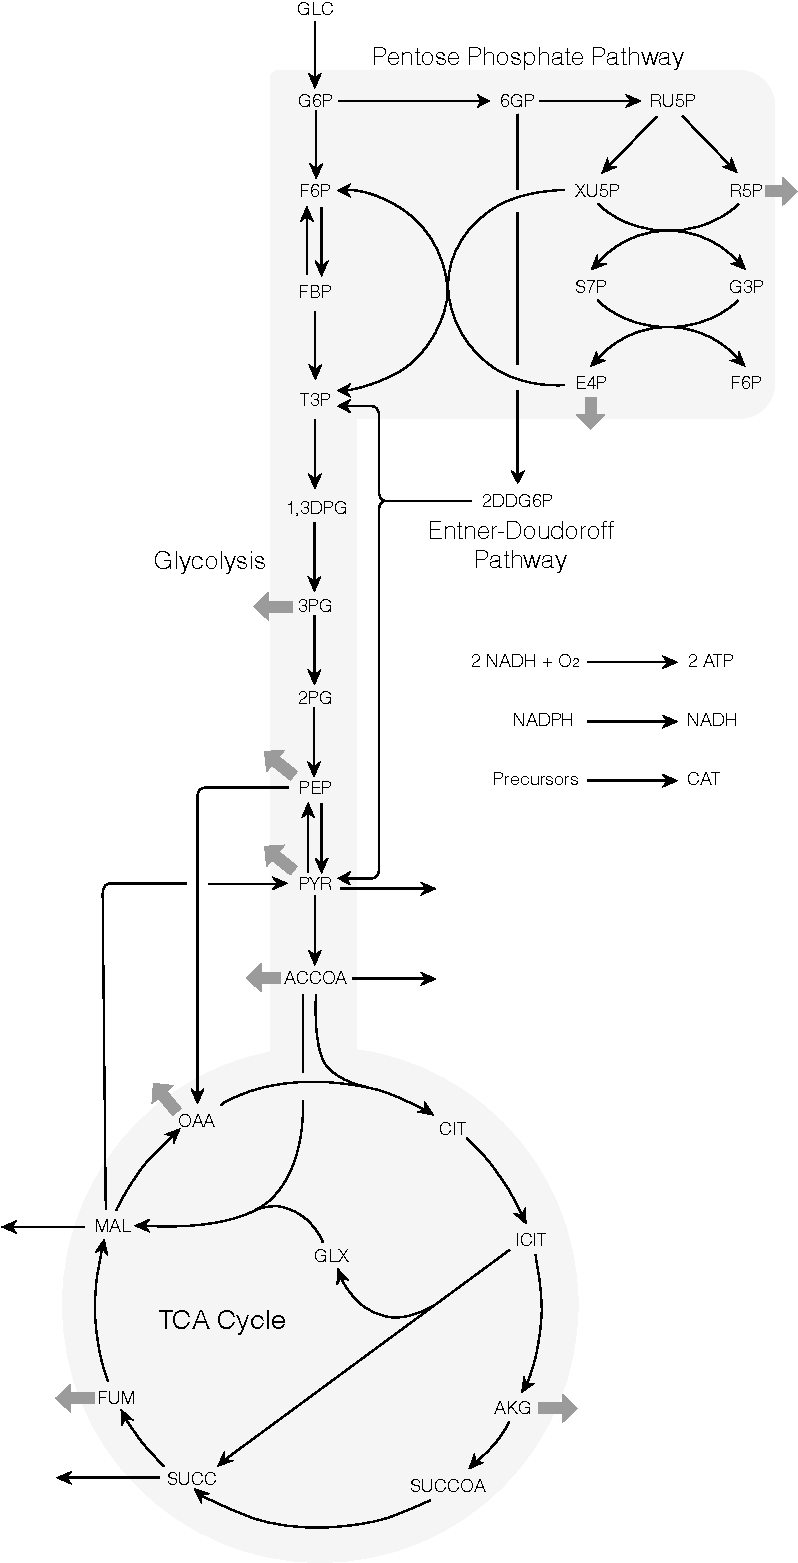
\includegraphics[width=0.75\textwidth]{./Figures/Network.pdf}
\caption{Flux profile for glycolysis, pentose phosphate pathway, Entner-Doudoroff pathway, TCA cycle, and NADPH/NADH transfer. Mean ± standard error for the reaction flux at 1.5 hrs (top) and 3 hrs (bottom), normalized to CAT synthesis flux.}
\label{fig:Network}
\end{figure}

\begin{figure}[ht]
\centering
%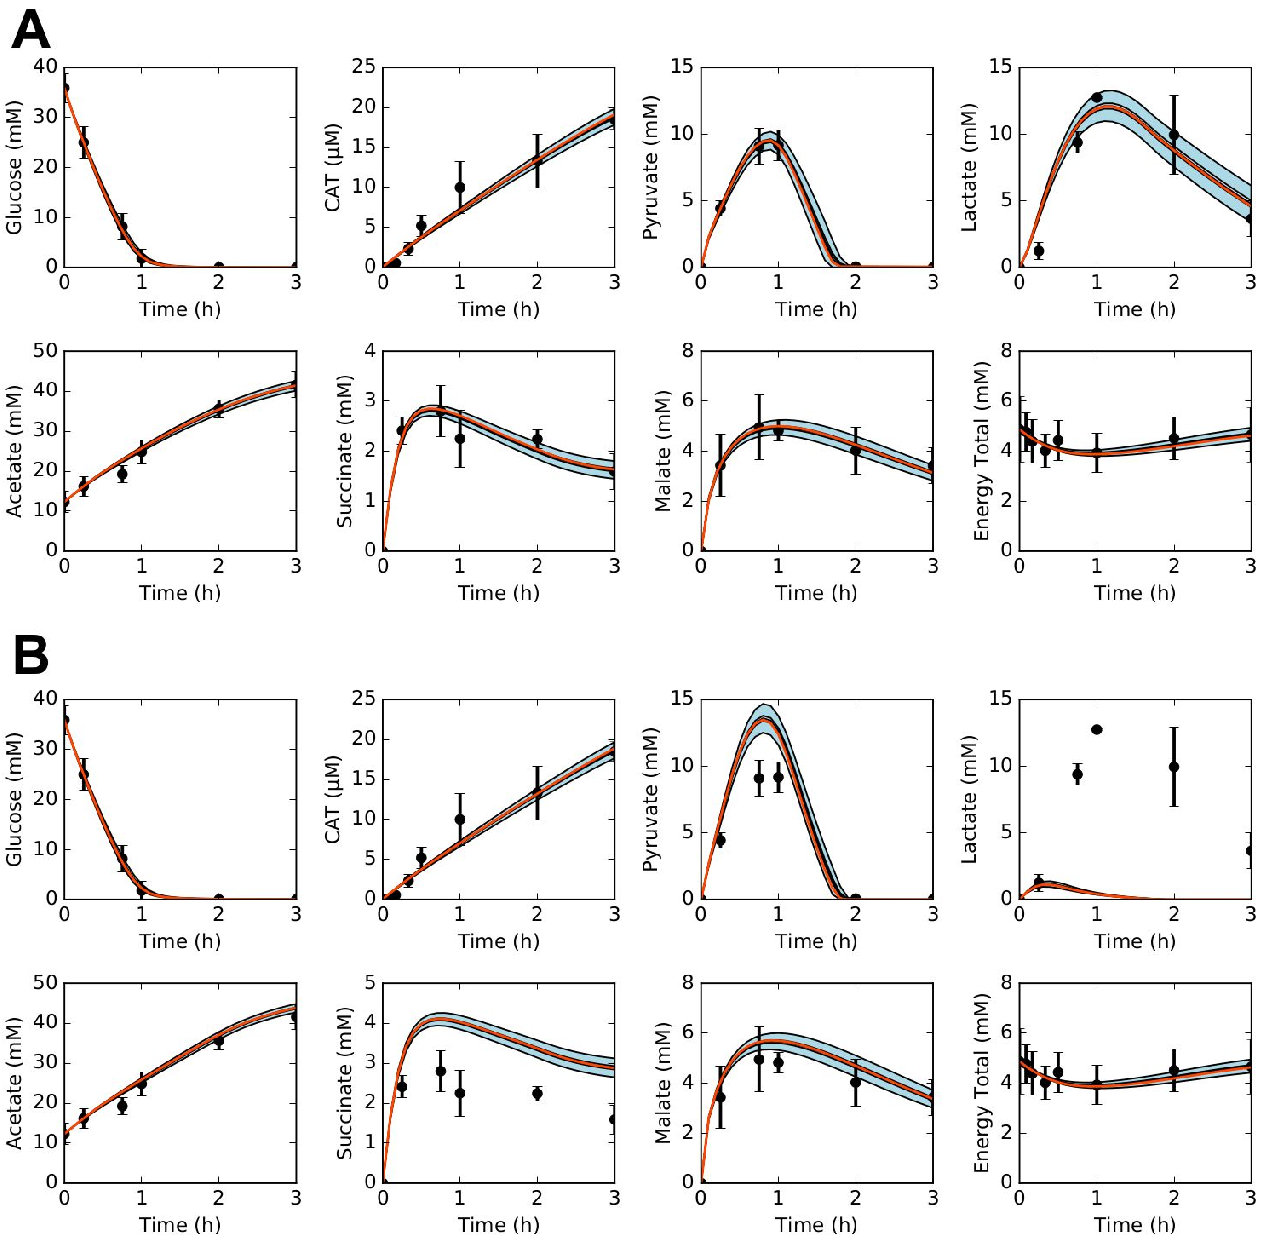
\includegraphics[width=1.00\textwidth]{./Figures/BothCarbon.pdf}
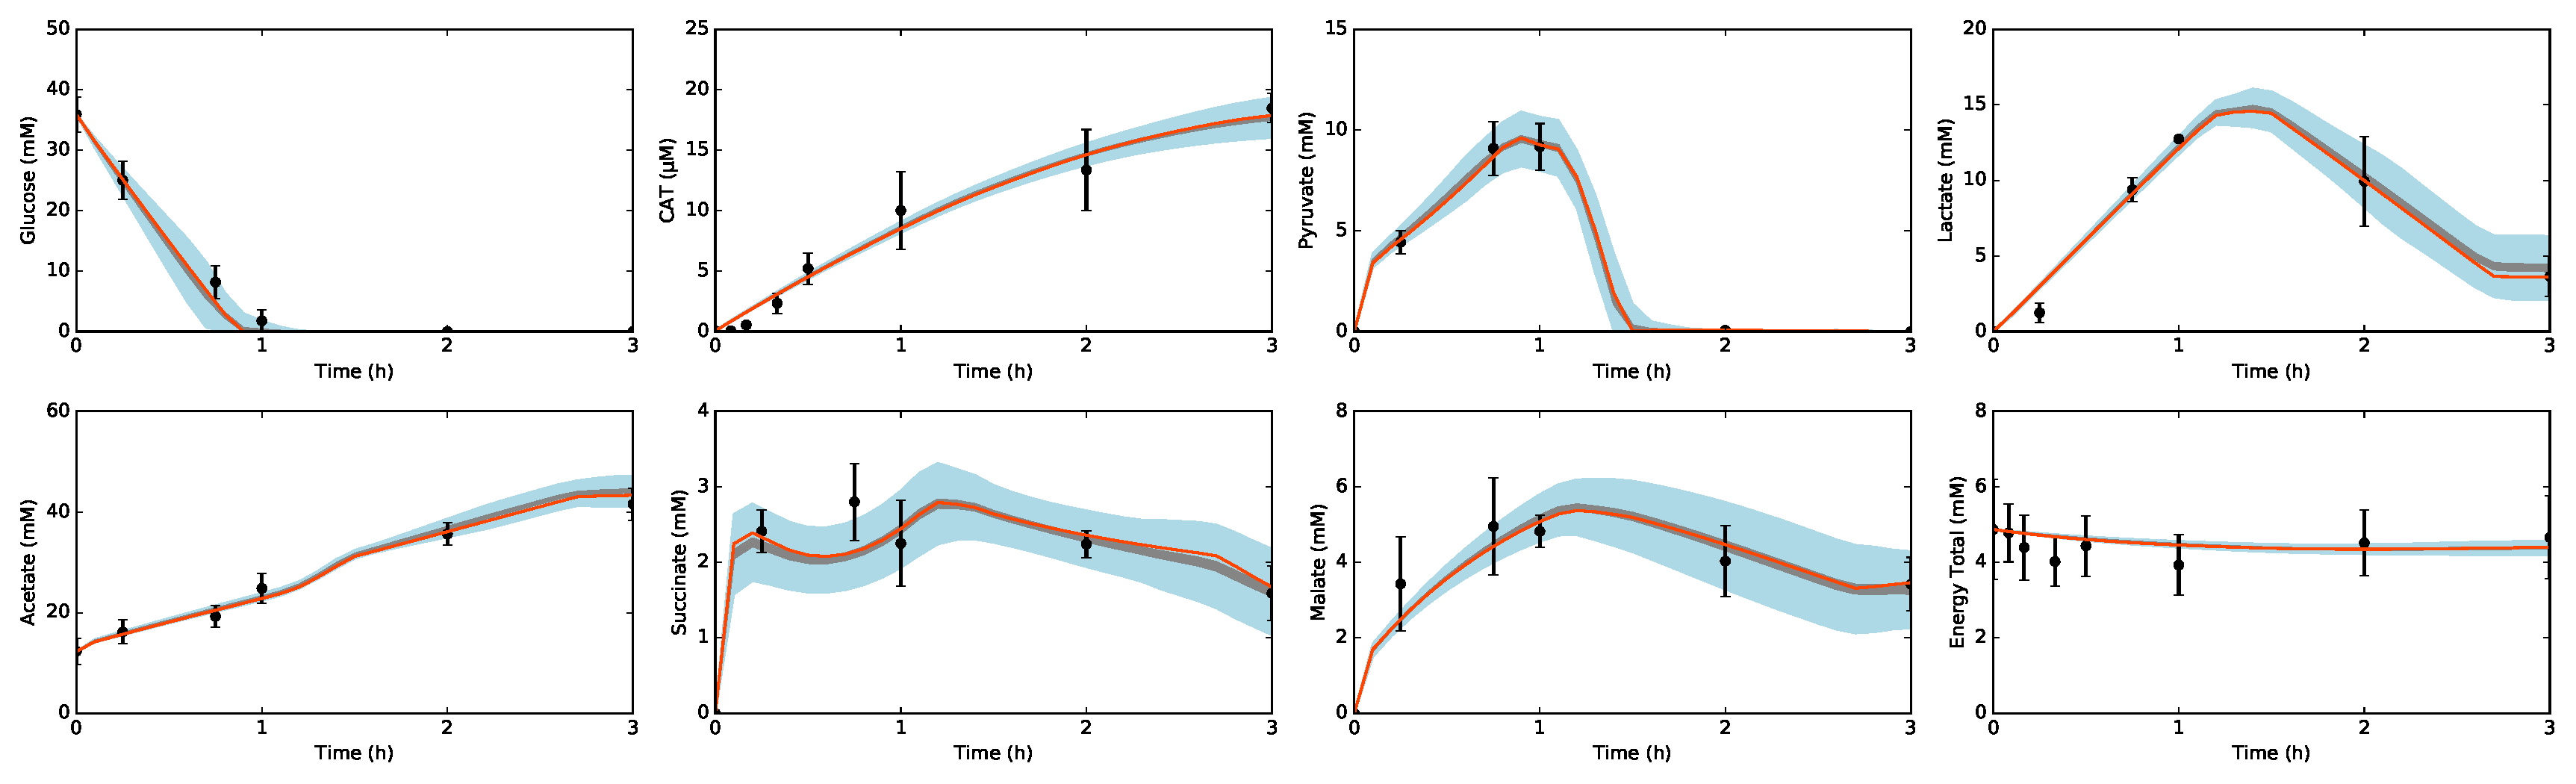
\includegraphics[width=1.00\textwidth]{./Figures/Carbon.pdf}

\includegraphics[width=0.05\textwidth]{./Figures/null.pdf}
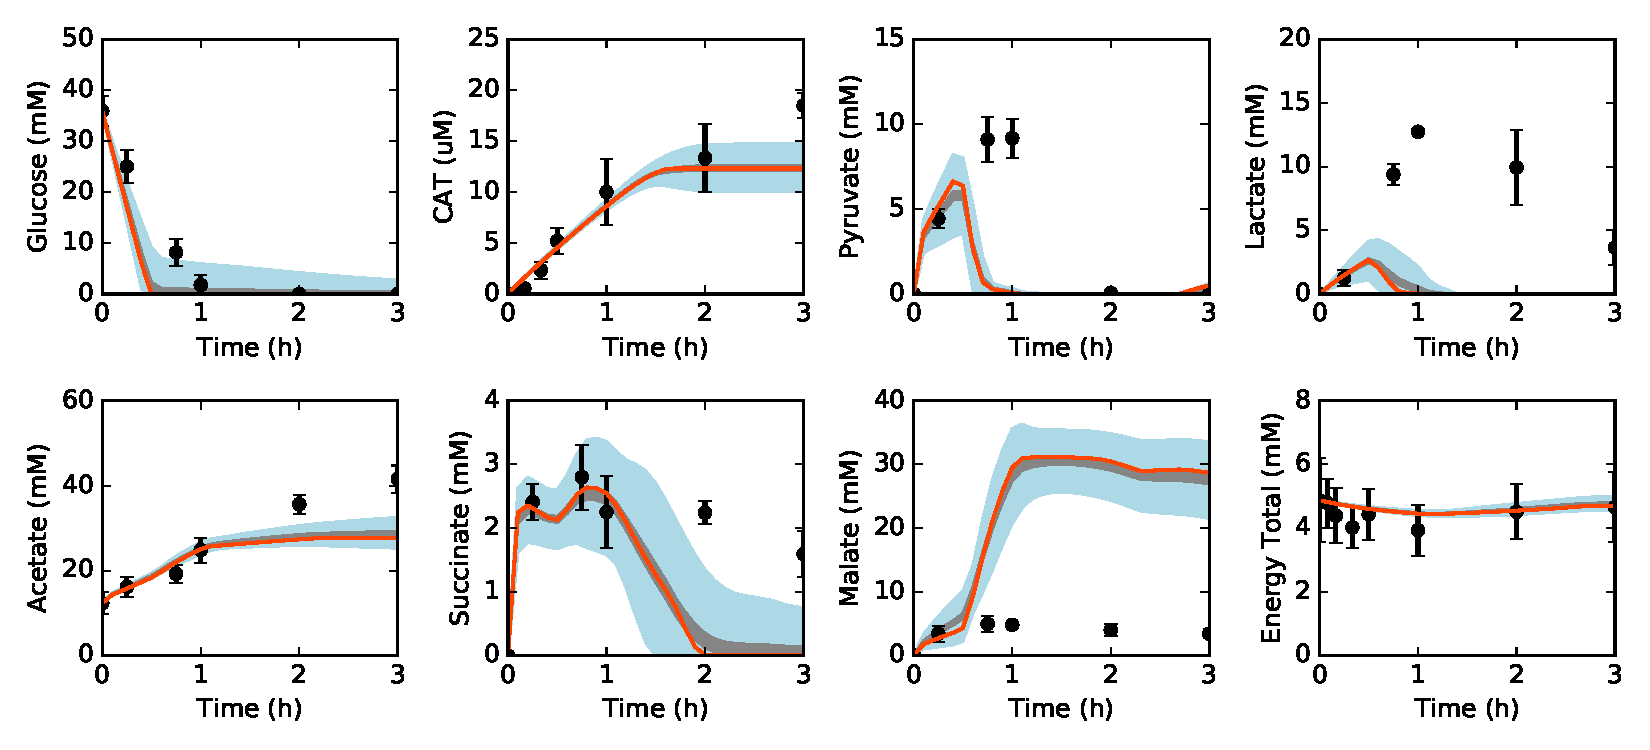
\includegraphics[width=1.00\textwidth]{./Figures/CarbonNoControl.pdf}
\caption{A: Central carbon metabolism in the presence of allosteric control, including glucose (substrate), CAT (product), and intermediates, as well as total concentration of energy species. Best-fit parameter set (orange line) versus experimental data (points). 95\% confidence interval (blue shaded region) and 95\% confidence interval of the mean (gray shaded region) over the ensemble of 18,000 sets. B: Central carbon metabolism in the absence of allosteric control.}
\label{fig:BothCarbon}
\end{figure}

\begin{figure}[ht]
\centering
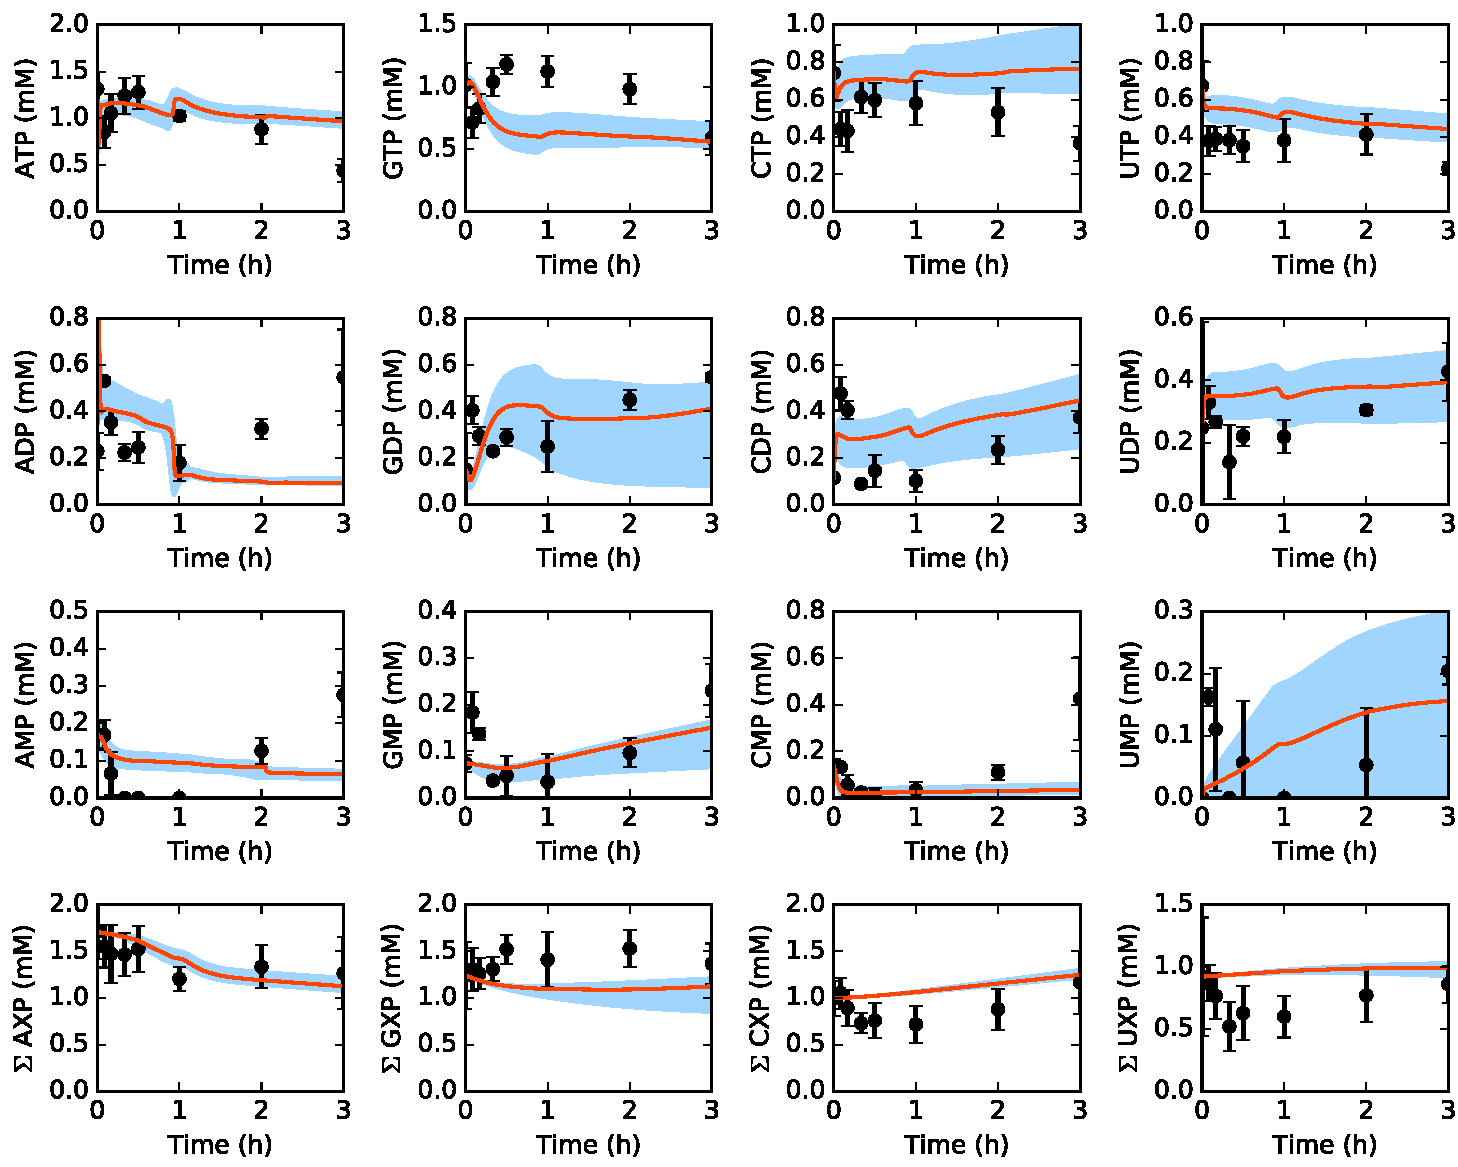
\includegraphics[width=1.00\textwidth]{./Figures/Energy.pdf}
\caption{Energy species and energy totals by base in the presence of allosteric control. Best-fit parameter set (orange line) versus experimental data (points). 95\% confidence interval (blue shaded region) and 95\% confidence interval of the mean (gray shaded region) over the ensemble of 18,000 sets.}
\label{fig:Energy}
\end{figure}

\begin{figure}[ht]
\centering
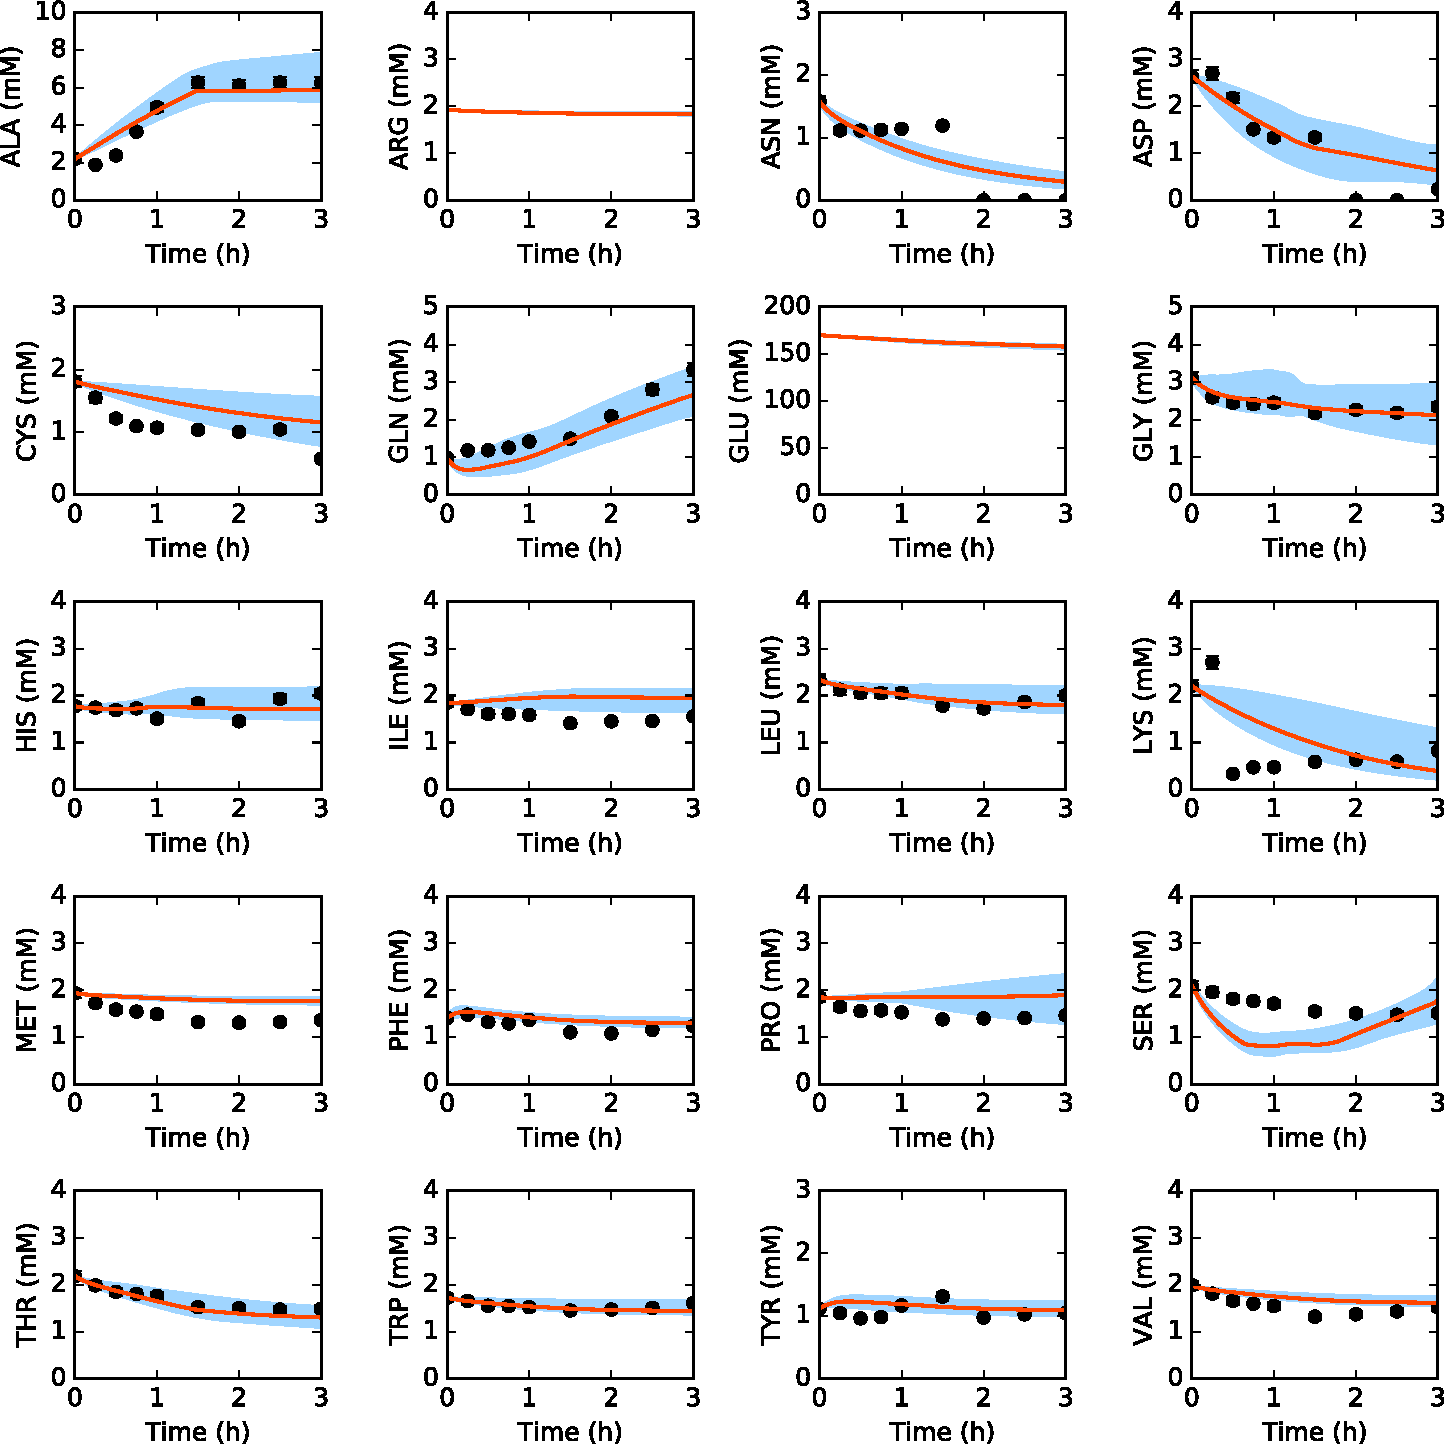
\includegraphics[width=1.00\textwidth]{./Figures/Amino.pdf}
\caption{Amino acids in the presence of allosteric control. Best-fit parameter set (orange line) versus experimental data (points). 95\% confidence interval (blue shaded region) and 95\% confidence interval of the mean (gray shaded region) over the ensemble of 18,000 sets.}
\label{fig:Amino}
\end{figure}

\begin{figure}[ht]
\centering
%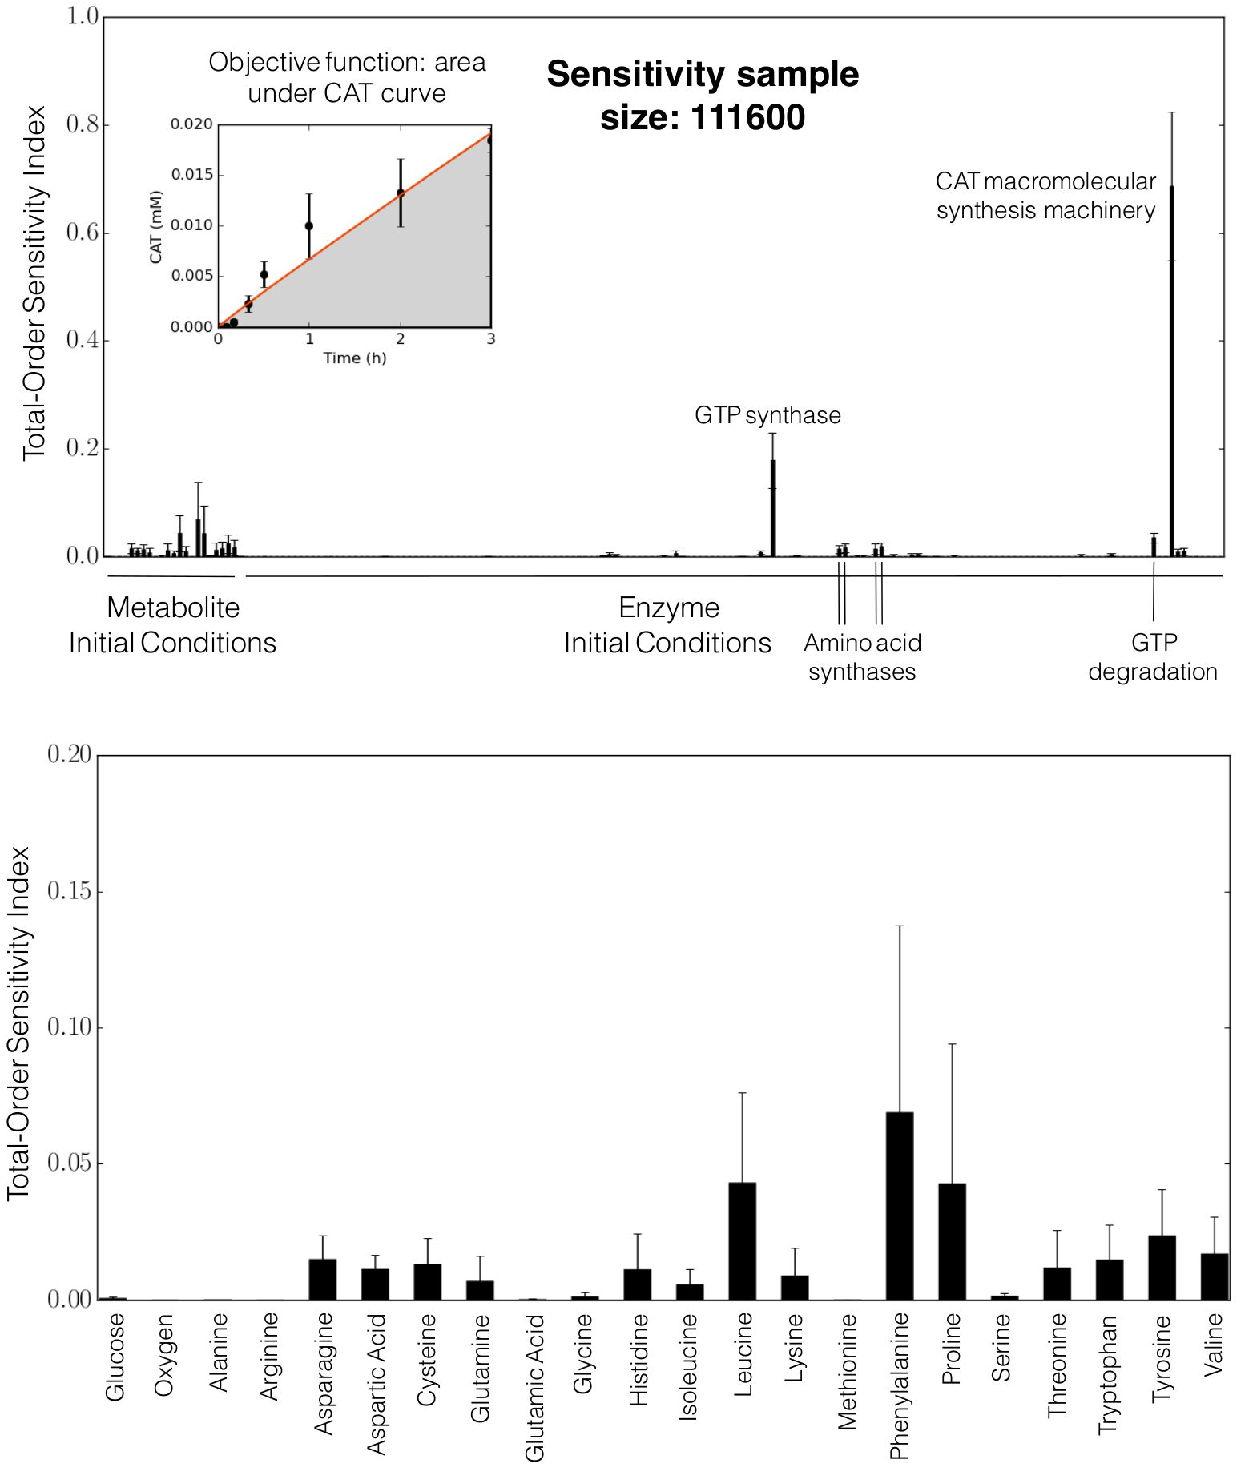
\includegraphics[width=1.00\textwidth]{./Figures/SensitivitiesHalfTall.pdf}
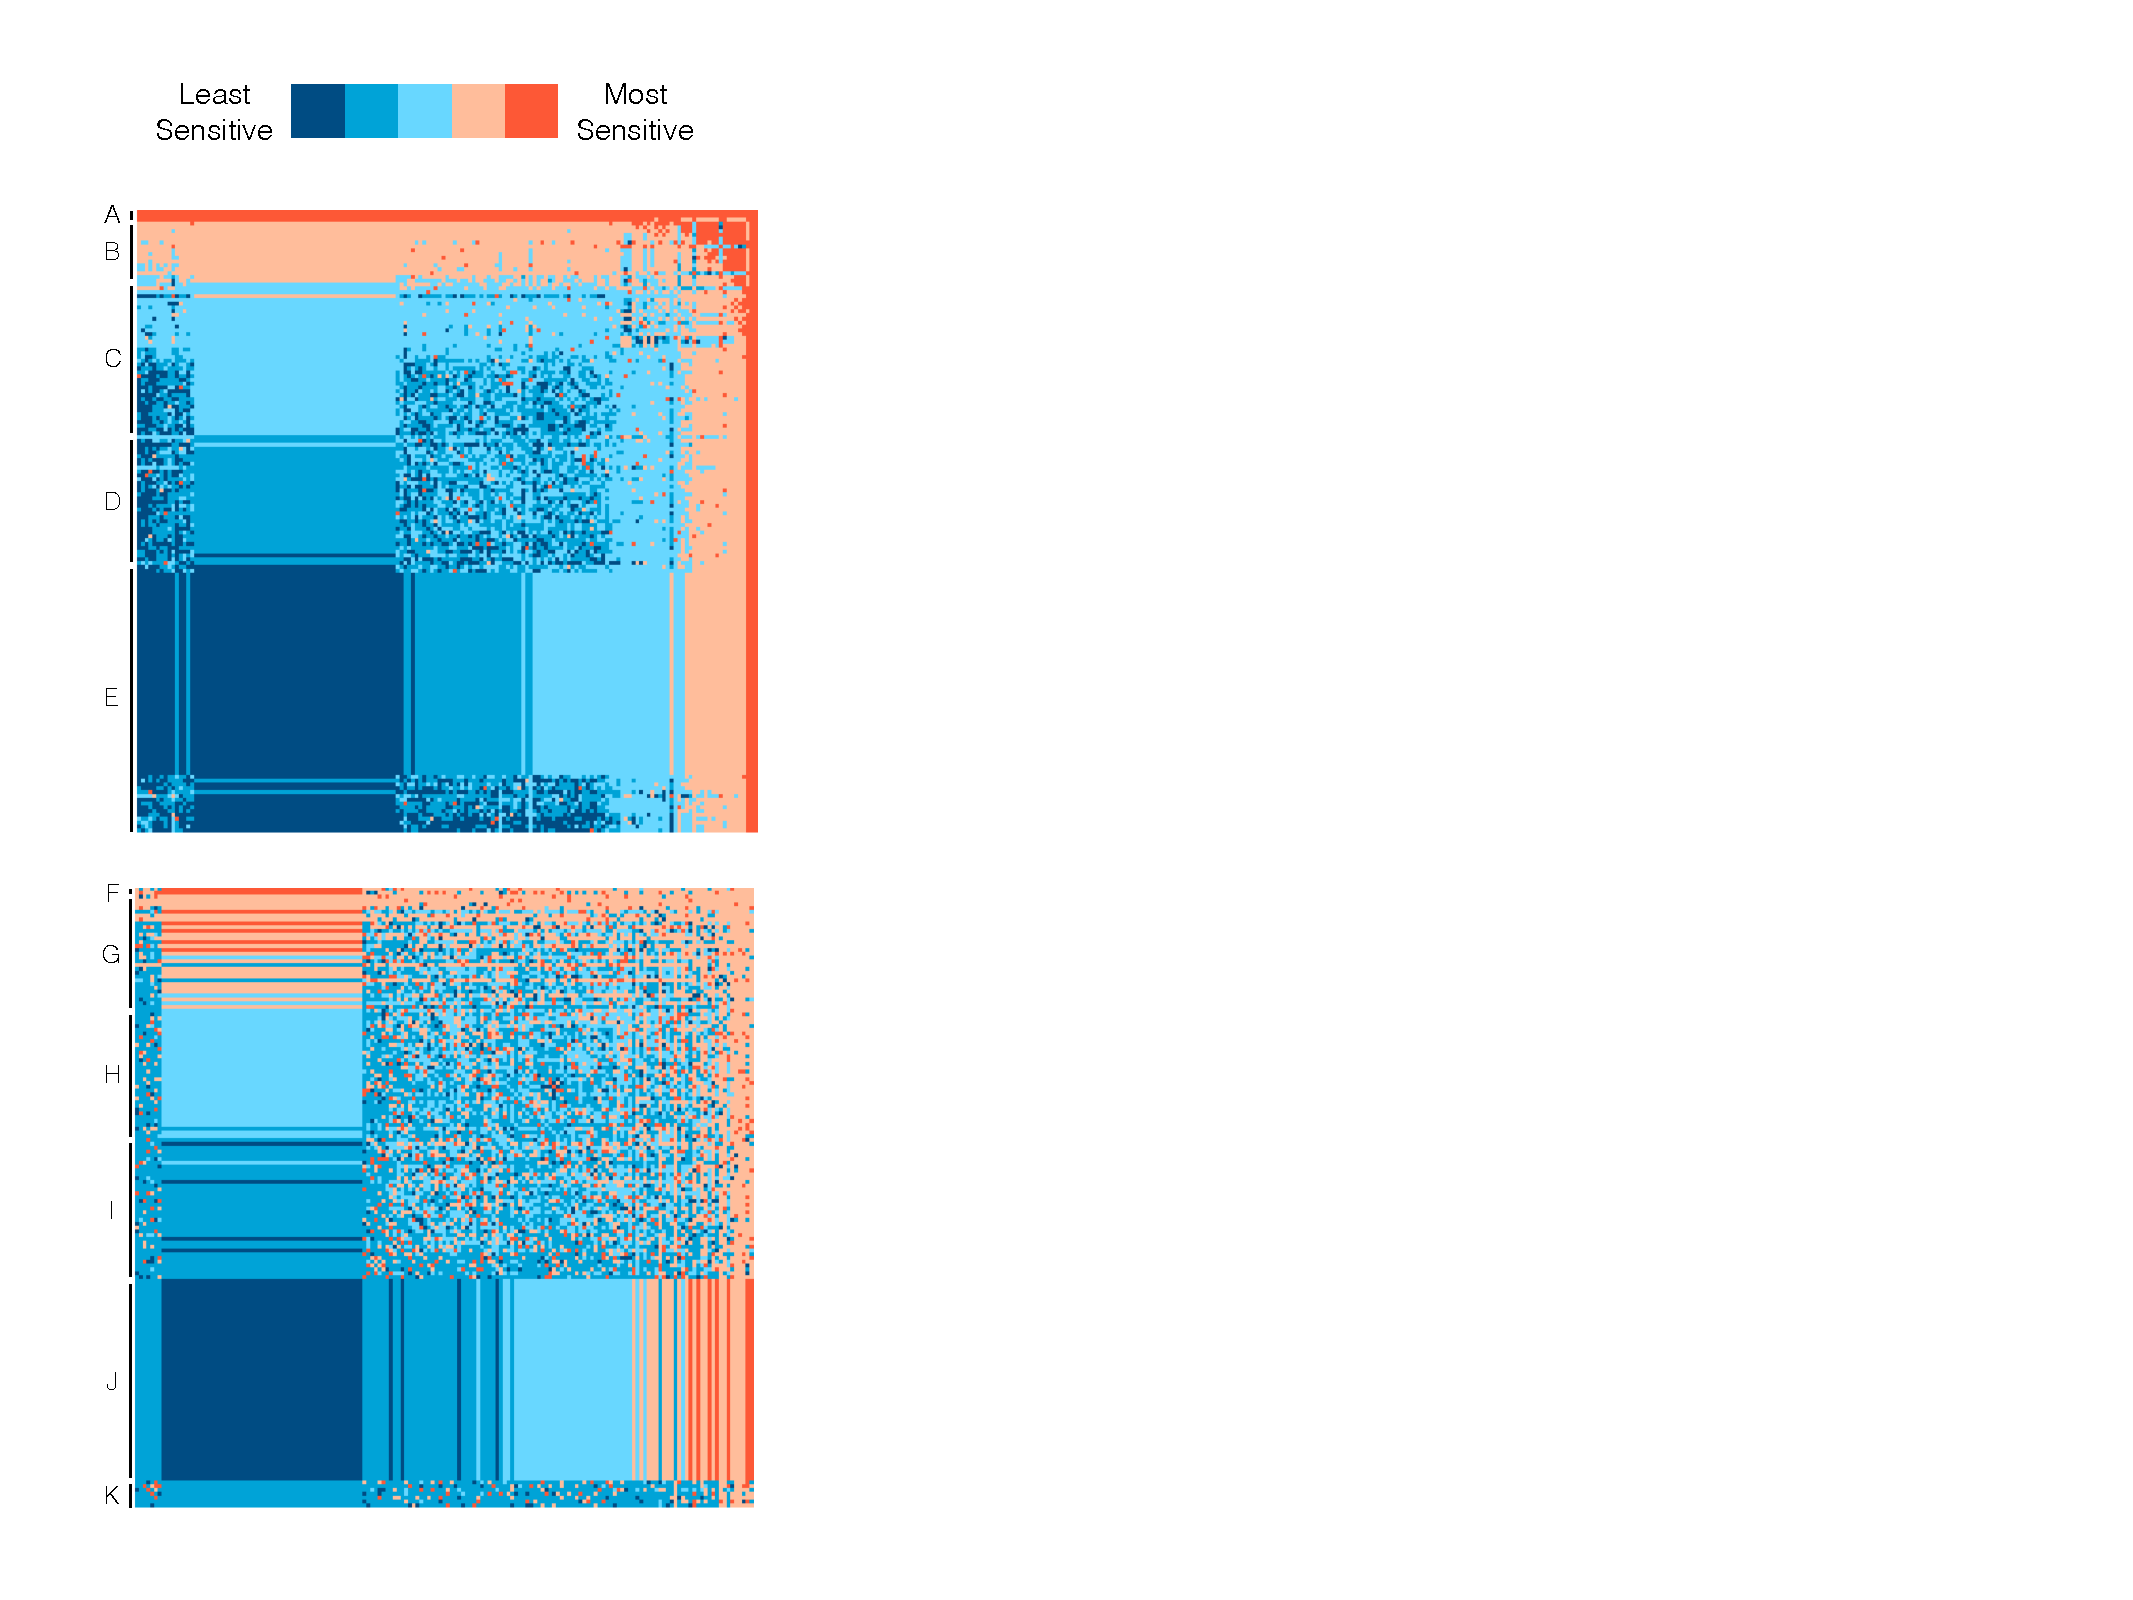
\includegraphics[width=1.00\textwidth]{./Figures/Sensitivity.pdf}
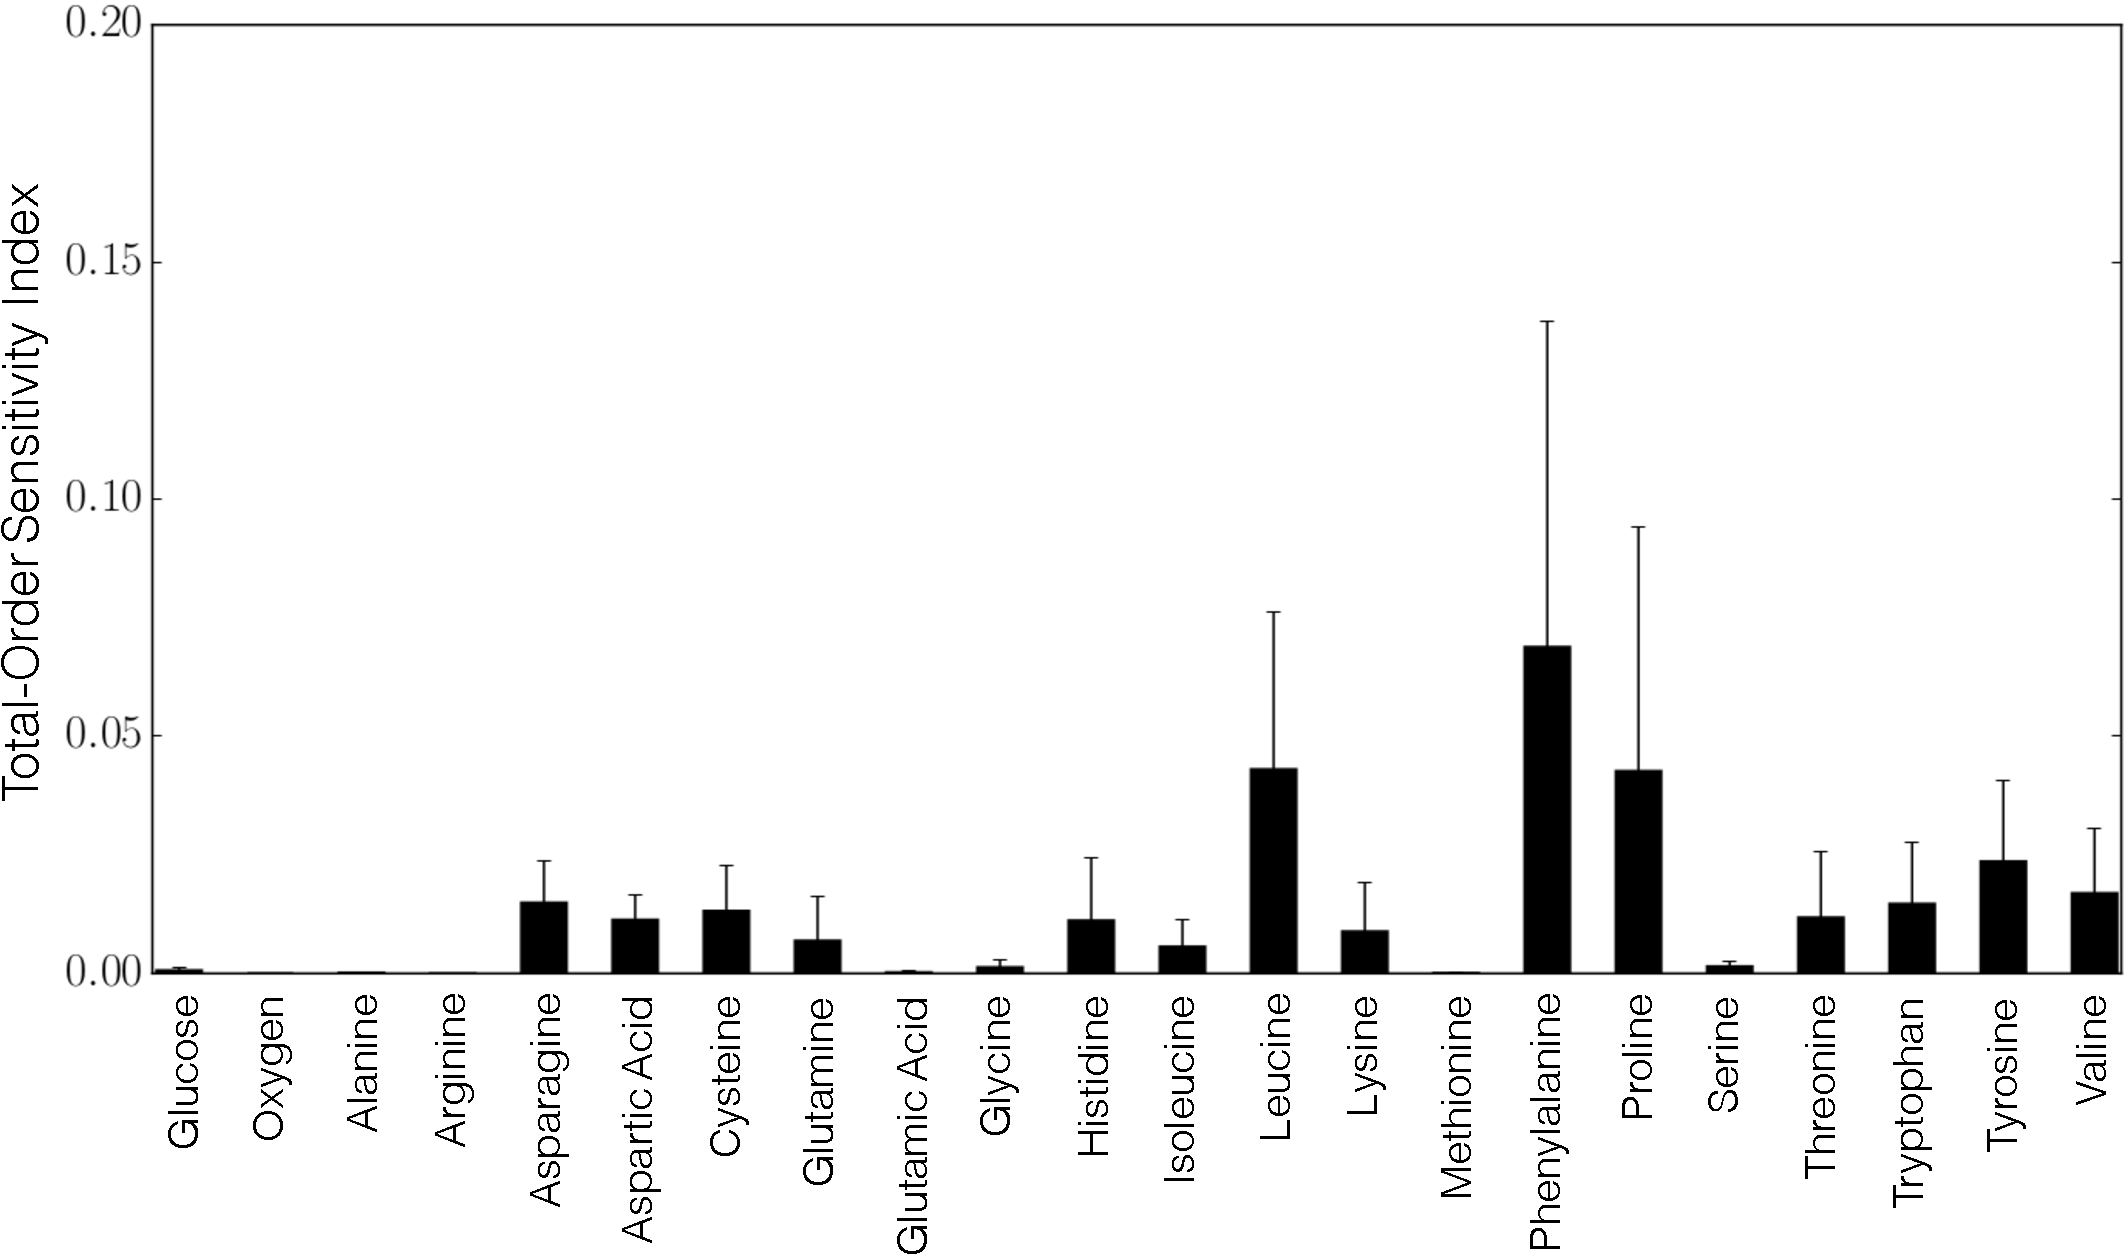
\includegraphics[width=1.00\textwidth]{./Figures/Metab_sensitivity.pdf}
\caption{Total-order global sensitivities for experimentally controllable initial conditions, including glucose, oxygen, amino acids, and enzymes.}
\label{fig:SensitivitiesHalfTall}
\end{figure}

\begin{figure}[ht]
\centering
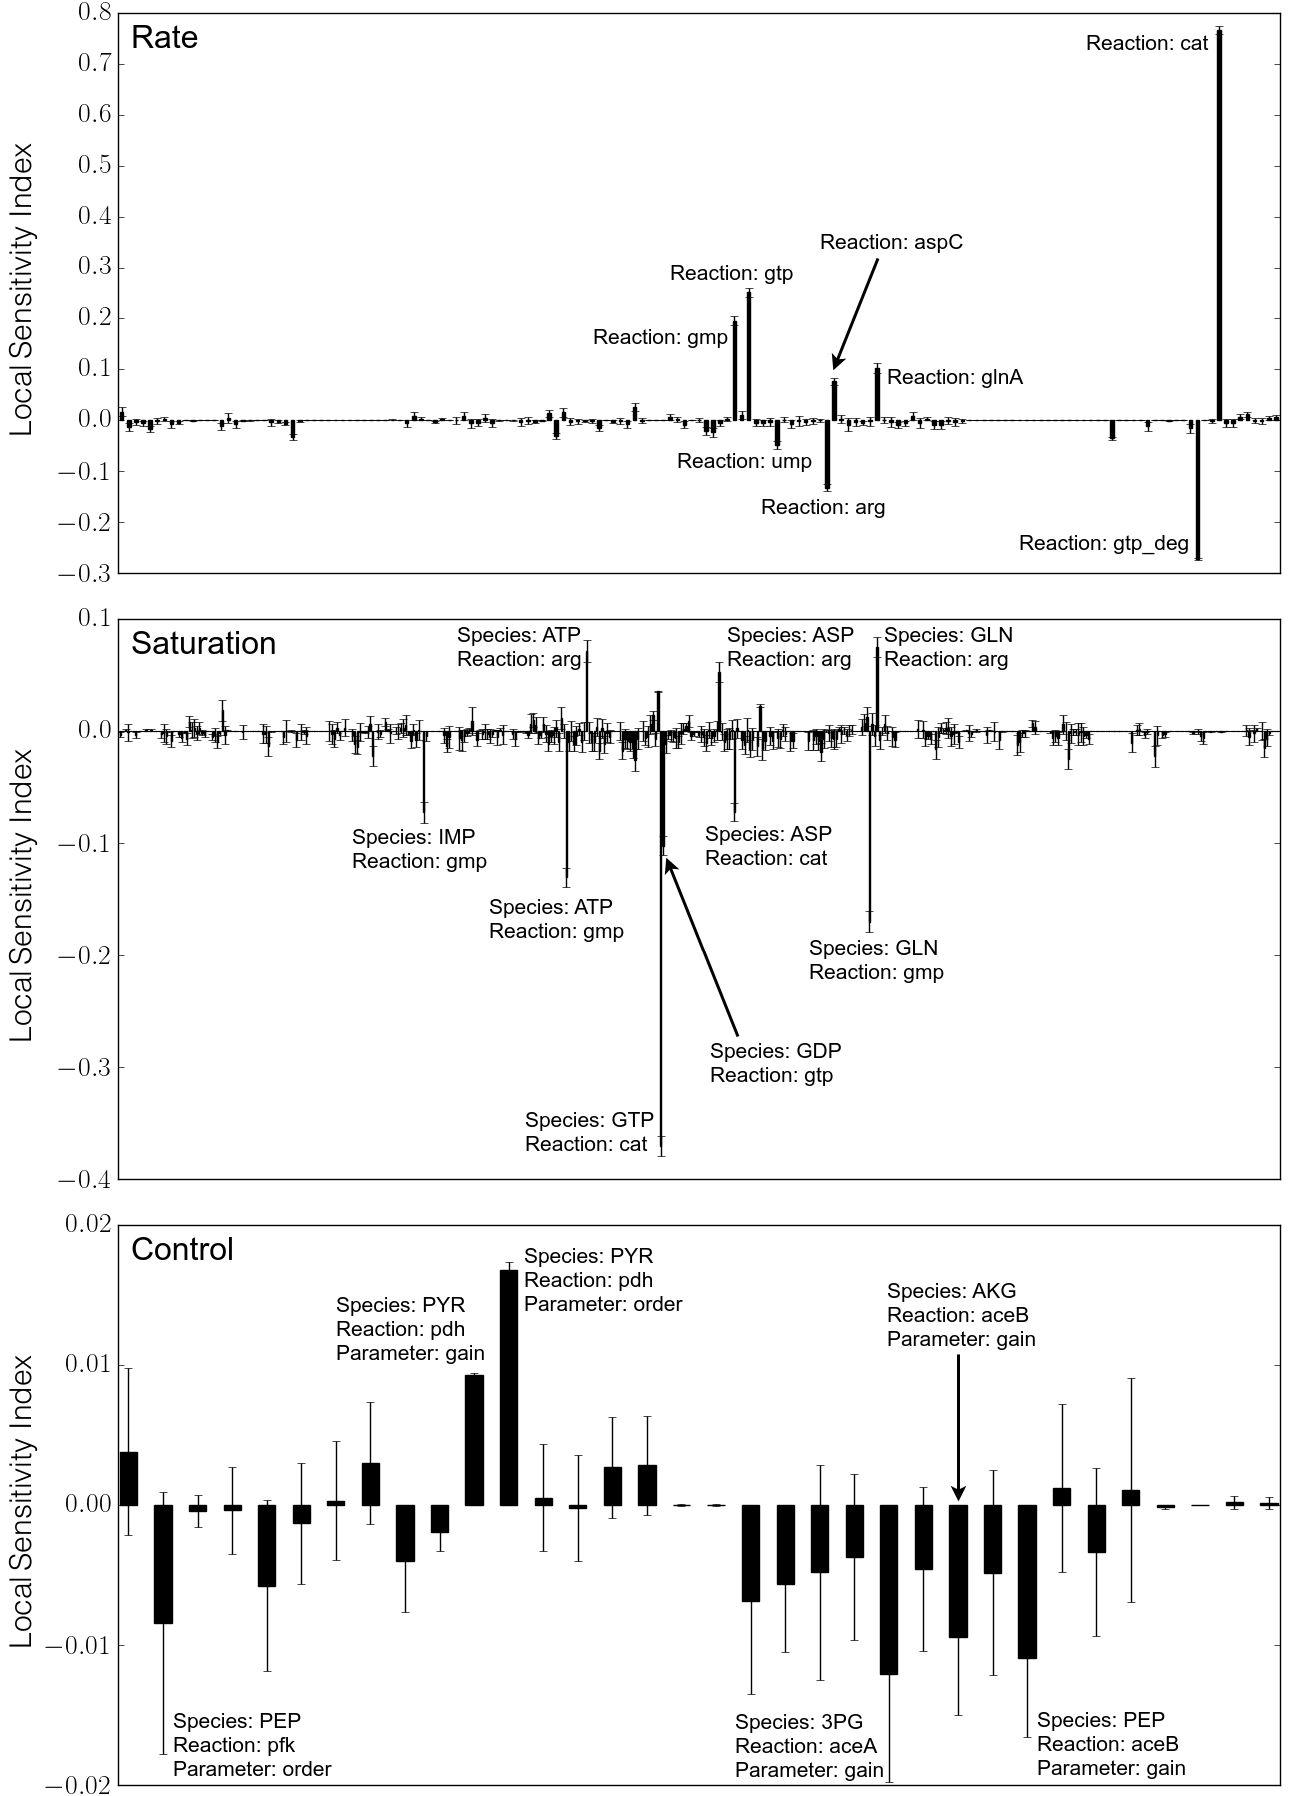
\includegraphics[width=0.94\textwidth]{./Figures/SensAll.png}
\caption{Mean and standard error of local sensitivities of rate constants (top), saturation constants (middle), and control parameters (bottom).}
\label{fig:SensAll}
\end{figure}

\clearpage

% Supplemental figures -
% Set the S-
\renewcommand\thefigure{S\arabic{figure}}
\renewcommand\thetable{T\arabic{table}}
\renewcommand\thepage{S-\arabic{page}}
\renewcommand\theequation{S\arabic{equation}}

% Reset the counters -
\setcounter{equation}{0}
\setcounter{table}{0}
\setcounter{figure}{0}
\setcounter{page}{1}


% Supplemental figures go here ...
%\begin{figure}[ht]
%\centering
%\includegraphics[width=1.00\textwidth]{./figs/<Filename>.pdf}
%\caption{Captiontext goes here}
%}\label{fig:<label_name>}
%\end{figure}

\end{document}
